% =============================================================================
% 09-efficient-sorting-notes.tex — Lecture Notes for Week 9:
% Beyond the Quadratic Wall (Efficient Sorting & the Comparison Lower Bound)
%
% DERIVED ARTIFACT. Source of truth:
% Slides/CS301/09-efficient-sorting.tex (55 pp incl. title/transitions).
% Generated by /lecture-notes at the "textbook-candidate prose" Detail Bar
% (every trace step written out, every example fully solved, Exercises with a
% separate Solutions block, reading guidance per section); do not hand-edit
% content independently of the Beamer source without re-running /qa-notes
% afterward (single-source-of-truth.md).
%
% Page-grounding (inherited 1:1 from the deck header; no upgrades):
%   Sedgewick2011 Sec.2.2 (Mergesort, p.270), Sec.2.3 (Quicksort, p.288),
%   Sec.2.4 (Priority Queues / heapsort, p.308), Sec.5.1 (String Sorts /
%   radix, p.702), order-of-growth table p.187; Wirth2004 Sec.2.3.1
%   (diminishing increment, p.52), Sec.2.3.3 (partition sort, p.57),
%   Sec.2.3.5 (comparison, p.62), Sec.2.4.1 (straight merging, p.63);
%   Karumanchi2017 Ch.10 (Sorting, pp.504-546 PDF), Ch.7 (Heaps, pp.369-408
%   PDF, Sec.7.7). Aho-Hopcroft-Ullman Ch.8, Horowitz & Sahni Ch.7,
%   Knuth Vol.3, Neapolitan Ch.2 cited at chapter level only.
%   All nine TikZ diagrams are reused verbatim from the deck.
%
% Compile with (macOS/Linux, ':'-joined TEXINPUTS/BIBINPUTS): cd Notes/CS301 &&
%   TEXINPUTS=../../Preambles:$TEXINPUTS xelatex -interaction=nonstopmode 09-efficient-sorting-notes.tex
%   BIBINPUTS=../..:$BIBINPUTS bibtex 09-efficient-sorting-notes
%   TEXINPUTS=../../Preambles:$TEXINPUTS xelatex -interaction=nonstopmode 09-efficient-sorting-notes.tex  (x2)
% =============================================================================

\documentclass[11pt]{article}
\usepackage[margin=1in]{geometry}
% =============================================================================
% Preambles/header.tex — shared LaTeX/Beamer preamble for this project
%
% Use from a Beamer lecture by prepending:
%     \input{header}
% and compiling with TEXINPUTS=../Preambles:$TEXINPUTS (the /compile-latex
% skill does this automatically).
%
% PALETTE CONTRACT. Color names defined here MUST match the names in
% Quarto/theme-template.scss so Beamer and Quarto renderings use the same
% palette. The scripts/check-palette-sync.sh script enforces this.
%
% To customize: edit the HEX values below AND the matching $variable in
% Quarto/theme-template.scss, then run scripts/check-palette-sync.sh.
% =============================================================================

% -----------------------------------------------------------------------------
% Engine detection + encoding
%
% Our /compile-latex skill uses XeLaTeX, where inputenc is unnecessary and
% can produce encoding warnings. Only load inputenc under pdfTeX.
% -----------------------------------------------------------------------------
\usepackage{iftex}
\ifPDFTeX
  \usepackage[utf8]{inputenc}
\fi

\usepackage{amsmath, amssymb, amsthm}
\usepackage{booktabs}
\usepackage{graphicx}

% -----------------------------------------------------------------------------
% PALETTE — mirrors Quarto/theme-template.scss variable names.
% Load xcolor and define colors BEFORE anything that references them
% (notably hyperref, hypersetup, and the Beamer color assignments).
% -----------------------------------------------------------------------------
\usepackage{xcolor}

\definecolor{primary-blue}{HTML}{012169}      % headings, accents
\definecolor{primary-gold}{HTML}{B9975B}      % emphasis, borders
\definecolor{highlight-yellow}{HTML}{F2A900}  % markers, alerts
\definecolor{light-bg}{HTML}{E8EDF5}          % title / section backgrounds
\definecolor{jet}{HTML}{1A1A1A}               % body text

% Semantic colors (used in diagrams and annotations)
\definecolor{positive}{HTML}{15803D}          % good / observed / identified
\definecolor{negative}{HTML}{B91C1C}          % bad / problematic / bias
\definecolor{neutral}{HTML}{525252}           % reference / context

% Highlight accents (match .hi-* classes in the SCSS)
\definecolor{hi-slate}{HTML}{314F4F}
\definecolor{hi-green}{HTML}{2E8B57}
\definecolor{hi-red}{HTML}{C41E3A}

% Semantic aliases so skill templates and snippets can write
% \textcolor{accent}{...} without hard-coding "primary-blue".
\colorlet{accent}{primary-blue}
\colorlet{accent2}{primary-gold}

% -----------------------------------------------------------------------------
% Hyperref — loaded AFTER xcolor + palette so link colors resolve.
% -----------------------------------------------------------------------------
\usepackage{hyperref}
\hypersetup{colorlinks=true, linkcolor=primary-blue, urlcolor=primary-blue,
            citecolor=primary-blue, pdfborder={0 0 0}}

% -----------------------------------------------------------------------------
% Course code — set once per deck (after \input{header}, before \begin{document})
% via \coursecode{CS401}. Shown in the footer on every slide so a deck's course
% is identifiable without opening the title page. Empty by default.
% -----------------------------------------------------------------------------
\makeatletter
\newcommand{\coursecode}[1]{\gdef\@coursecodetext{#1}}
\gdef\@coursecodetext{}
\makeatother

% -----------------------------------------------------------------------------
% Beamer theme assignments (only apply under Beamer).
%
% We detect Beamer via \@ifclassloaded{beamer}, which is the documented,
% non-internal way. This must be wrapped in \makeatletter/\makeatother
% because \@ifclassloaded contains an @-catcode character.
% -----------------------------------------------------------------------------
\makeatletter
\@ifclassloaded{beamer}{%
  \usefonttheme{professionalfonts}
  \setbeamercolor{structure}{fg=primary-blue}
  \setbeamercolor{frametitle}{fg=primary-blue}
  \setbeamercolor{title}{fg=primary-blue}
  \setbeamercolor{subtitle}{fg=primary-gold}
  \setbeamercolor{author}{fg=primary-blue}
  \setbeamercolor{institute}{fg=neutral}
  \setbeamercolor{date}{fg=primary-gold}
  \setbeamercolor{itemize item}{fg=primary-blue}
  \setbeamercolor{itemize subitem}{fg=primary-gold}
  \setbeamercolor{alerted text}{fg=primary-gold}
  \setbeamercolor{block title}{fg=white, bg=primary-blue}
  \setbeamercolor{block body}{bg=light-bg}
  % Semantic block variants: block=definition/concept (blue), exampleblock=
  % worked example (green/positive), alertblock=key takeaway or caution (gold).
  % Keep to <=2 colored boxes per slide across ALL three variants (INV-7).
  \setbeamercolor{block title example}{fg=white, bg=positive}
  \setbeamercolor{block body example}{bg=light-bg}
  \setbeamercolor{block title alerted}{fg=white, bg=primary-gold}
  \setbeamercolor{block body alerted}{bg=light-bg}

  % Minimal footer: course code (left) + page X / N (right), no navigation clutter
  \setbeamertemplate{navigation symbols}{}
  \setbeamertemplate{footline}{%
    \color{neutral}\footnotesize\hspace{0.7em}\@coursecodetext\hfill
    \insertframenumber/\inserttotalframenumber\hspace{0.7em}\vspace{0.3em}}
}{}
\makeatother

% -----------------------------------------------------------------------------
% TikZ setup — libraries the snippet gallery uses
% -----------------------------------------------------------------------------
\usepackage{tikz}
\usetikzlibrary{arrows.meta, positioning, calc, decorations.pathreplacing,
                fit, shapes.geometric, backgrounds}

% Shared TikZ styles — snippets and hand-written diagrams can pick these up
% via `\begin{tikzpicture}[every node/.style={...}]` or by naming specific
% styles (e.g., `\node[dag-node] (X) at (0,0) {X};`).
\tikzset{
  % Node styles for causal DAGs and similar
  dag-node/.style = {
    draw=primary-blue, fill=light-bg, rounded corners=2pt,
    minimum width=1.2cm, minimum height=0.9cm, align=center, font=\small
  },
  decision-node/.style = {
    draw=primary-gold, fill=white, diamond, aspect=1.8,
    minimum width=1.8cm, minimum height=1.2cm, align=center, font=\small,
    inner sep=1pt
  },
  % Edge styles — observed vs counterfactual
  observed-edge/.style = {-{Latex[length=2.5mm]}, thick, draw=jet},
  counterfactual-edge/.style = {-{Latex[length=2.5mm]}, thick, draw=neutral, dashed},
  confound-edge/.style = {-{Latex[length=2.5mm]}, thick, draw=negative, dashed},
  % Data-point styles for plots
  observed-dot/.style = {fill=primary-blue, draw=primary-blue, circle, inner sep=1.2pt},
  counterfactual-dot/.style = {fill=white, draw=neutral, circle, inner sep=1.2pt}
}

% -----------------------------------------------------------------------------
% Convenience macros
% -----------------------------------------------------------------------------
\newcommand{\muted}[1]{\textcolor{neutral}{#1}}
\newcommand{\key}[1]{\textcolor{primary-gold}{\textbf{#1}}}
\newcommand{\good}[1]{\textcolor{positive}{#1}}
\newcommand{\bad}[1]{\textcolor{negative}{#1}}

% Standout frame macro: full-bleed dark background for section transitions.
% Beamer-only (uses \begin{frame}/\setbeamercolor/\usebeamerfont) -- do not
% call from an article-class file (e.g. Notes/<CODE>/*-notes.tex). \muted,
% \key, \good, \bad, and \coursecode above are plain xcolor/gdef and are
% safe to use from either class; verified when Notes/article-class support
% was added.
% Expand: \transitionslide{Your transition title}
\newcommand{\transitionslide}[1]{%
  \begingroup
  \setbeamercolor{background canvas}{bg=primary-blue}
  \begin{frame}[plain]
    \centering
    \vfill
    {\usebeamerfont{title}\color{white}\Large #1\par}
    \vfill
  \end{frame}
  \endgroup
}

% Section divider frame (Beamer-only), an alternative to \transitionslide with a
% darker two-line style: near-black (jet) background, a small white label line
% above a larger gold title, and a thin gold rule along the bottom edge.
% Expand: \sectiondivider{Section 2}{Pointers}
\newcommand{\sectiondivider}[2]{%
  \begingroup
  \setbeamercolor{background canvas}{bg=jet}
  \begin{frame}[plain]
    \vspace*{3.0cm}
    {\color{white}\ttfamily\large #1\par}
    \vspace{0.5cm}
    {\color{primary-gold}\LARGE #2\par}
    \begin{tikzpicture}[remember picture, overlay]
      \draw[primary-gold, line width=2.5pt]
        ($(current page.south west)+(0,0.1)$) -- ($(current page.south east)+(0,0.1)$);
    \end{tikzpicture}
  \end{frame}
  \endgroup
}

% -----------------------------------------------------------------------------
% Channel watermark — "Concepts That Click" (YouTube).
%
% Article-class files (CompetitiveExam Q/A sets, Notes, Assignments) get a
% light diagonal draft watermark on every page plus a centered footer naming
% the channel. Beamer decks get a subtle TikZ background watermark instead
% (the footline already carries the course code). Centralized here so every
% MCQ PDF is branded without per-file edits.
% -----------------------------------------------------------------------------
\makeatletter
\@ifclassloaded{article}{%
  \usepackage{draftwatermark}
  \SetWatermarkText{Concepts That Click}
  \SetWatermarkScale{1}
  \SetWatermarkFontSize{2cm}
  \SetWatermarkLightness{0.86}
  \SetWatermarkAngle{45}
  \usepackage{fancyhdr}
  \pagestyle{fancy}
  \fancyhf{}
  \fancyfoot[C]{\footnotesize\textcolor{neutral}{Concepts That Click~|~YouTube: \href{https://www.youtube.com/@concepts.thatclick}{@concepts.thatclick}}}
  \renewcommand{\headrulewidth}{0pt}
  \renewcommand{\footrulewidth}{0pt}
  \fancypagestyle{plain}{%
    \fancyhf{}%
    \fancyfoot[C]{\footnotesize\textcolor{neutral}{Concepts That Click~|~YouTube: \href{https://www.youtube.com/@concepts.thatclick}{@concepts.thatclick}}}%
    \renewcommand{\headrulewidth}{0pt}%
    \renewcommand{\footrulewidth}{0pt}%
  }
}{}
\@ifclassloaded{beamer}{%
  \setbeamertemplate{background}{%
    \begin{tikzpicture}[remember picture, overlay]
      \node[rotate=45, opacity=0.055, align=center]
        at (current page.center)
        {\Huge\textcolor{neutral}{Concepts That Click}};
    \end{tikzpicture}%
  }
}{}
\makeatother 
\coursecode{CS301}

% Emergency stretch so long \texttt{} tokens in prose do not spill the margin.
\setlength{\emergencystretch}{2.5em}

% Chapter-style numbering: this is Week 9's chapter.
\renewcommand{\thesection}{9.\arabic{section}}
\renewcommand{\thefigure}{9.\arabic{figure}}
\newtheorem{example}{Example}[section]

\newenvironment{definitionbox}[1]{%
  \par\noindent\textbf{Definition (#1).}\ \itshape
}{\par\vspace{0.3em}}

\title{Beyond the Quadratic Wall\\\large Lecture Notes --- Week 9: Efficient Sorting \& the Comparison Lower Bound}
\author{Auqib Hamid Lone\\[0.3em]
  \small Department of Computer Science \& Engineering\\
  \small Government College of Engineering \& Technology (GCET), Ganderbal}
\date{\today}

\begin{document}
\maketitle

\section{Why This Week Exists: The Cost of Getting Sorted}

\textbf{Read alongside:} Sedgewick, \textit{Algorithms}, Sec.~2.2--2.4, pp.270--335 --- mergesort, quicksort, and heapsort with their analyses; Karumanchi, \textit{Data Structures and Algorithms Made Easy}, Ch.~10, pp.504--546 (PDF) --- the comparative treatment of merge, quick, shell, and radix sort.

Week~8 ended with a promise: having built the elementary sorts, the course would ask ``why can no \emph{comparison} sort beat $\Theta(n \log n)$, and which algorithms escape that bound?'' This chapter pays that promise off. It does not re-teach asymptotic notation (Week~2), array address arithmetic (Week~3), or the vocabulary of stability and in-place operation (Week~8); it uses all three.

The deficiency that motivates the week is concrete. The calculator's symbol table now holds $2{,}000$ identifiers. It is sorted once at startup and searched many times thereafter, so the sorting cost is a startup pause. Insertion sort pays about
\[
  \frac{n(n-1)}{2} = \frac{2{,}000 \times 1{,}999}{2} = 1{,}999{,}000
\]
comparisons in the worst case. A merge sort pays about $n\log_2 n = 2{,}000 \times 11 \approx 22{,}000$ --- roughly $91$ times fewer. At one million records the gap widens to roughly $25{,}000$ times. The elementary sorts are not wrong; they are priced for a different $n$.

The questions that organize the chapter are the deck's five: where the $\log$ in $n\log n$ comes from; whether a ceiling exists that no comparison sort can pass; how heap sort combines the guarantee with $O(1)$ space; how radix sort beats the bound; and where shell sort fits between insertion sort and quick sort.

\muted{Running application (Weeks 3--10): one calculator, rebuilt each week. Week 9 asks how its identifier table gets sorted fast enough to be worth sorting.}

\section{Divide and Conquer: Merge Sort}

\textbf{Read alongside:} Sedgewick, Sec.~2.2, pp.270--287 --- mergesort and its analysis; Wirth, Sec.~2.4.1, p.63 --- straight merging; Karumanchi, Ch.~10, pp.504--546 (PDF).

\subsection{The pattern and its three questions}

Sorting $2{,}000$ records in one pass is hard. Sorting two halves of $1{,}000$ is easier, and \emph{combining} two already-sorted halves is a single linear scan. This is the divide-and-conquer pattern: divide the input, conquer each part recursively, combine the answers.

\begin{definitionbox}{divide-and-conquer sorting \cite{AhoHopcroftUllman1983_data_structures_algorithms}}
A sorting algorithm is divide-and-conquer when it (1) splits the input into independent subproblems, (2) sorts each recursively, and (3) combines the sorted parts without re-examining any element more than a constant number of times. Its cost satisfies a recurrence of the form $T(n) = a\,T(n/b) + \Theta(\text{combine})$.
\end{definitionbox}

Merge sort answers the three questions directly. It splits at the midpoint, conquers the two halves, and combines them by \emph{merging} two sorted runs. Only the merge step is new machinery.

\subsection{The merge step}

\begin{definitionbox}{merge \cite{Sedgewick2011_algorithms,Wirth2004_algorithms_data_structures}}
\texttt{merge(A, lo, mid, hi)} requires $A[\texttt{lo}..\texttt{mid}]$ and $A[\texttt{mid}+1..\texttt{hi}]$ to be sorted. It rearranges the range so that $A[\texttt{lo}..\texttt{hi}]$ is sorted. On equal keys it takes the element from the \emph{left} run first, which is what makes the merge stable.
\end{definitionbox}

The mechanism is two fingers. Point one at the front of each run. Compare the two front elements, copy the smaller to the output, and advance that finger. When one run is exhausted, copy the rest of the other. Every element is copied exactly once, so merging a range of $n$ elements costs $\Theta(n)$.

\begin{example}
Merge $[3,8,15]$ with $[2,9,11]$. Compare $3$ and $2$: take $2$. Compare $3$ and $9$: take $3$. Compare $8$ and $9$: take $8$. Compare $15$ and $9$: take $9$. Compare $15$ and $11$: take $11$. The left run is exhausted, so drain $15$. The output is $[2,3,8,9,11,15]$. Five comparisons were needed --- at most $m+n-1$ for runs of lengths $m$ and $n$, because the last element is drained without a comparison.
\end{example}

\begin{figure}[h]
  \centering
  % Diagram: merging left run [3,8,15] with right run [2,9,11]. Each run is
  % a row of three cells; the output row below receives the smaller front
  % element. Coordinates: cells 0.9 cm wide at x = 0,1.1,2.2 (left) and
  % x = 3.6,4.7,5.8 (right); output cells at x = 0..5.5, y = -0.9.
  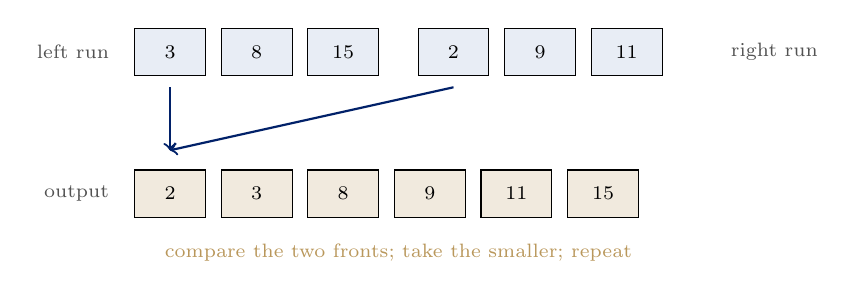
\begin{tikzpicture}[every node/.style={font=\scriptsize}]
    \foreach \i/\v in {0/3,1/8,2/15}
      \node[draw, fill=light-bg, minimum width=0.9cm,
        minimum height=0.6cm, align=center] (l\i) at (\i*1.1, 0.9) {\v};
    \foreach \i/\v in {0/2,1/9,2/11}
      \node[draw, fill=light-bg, minimum width=0.9cm,
        minimum height=0.6cm, align=center] (r\i) at (3.6+\i*1.1, 0.9) {\v};
    \node[anchor=east, text=neutral] at (-0.65, 0.9) {left run};
    \node[anchor=west, text=neutral] at (7.0, 0.9) {right run};
    \foreach \i/\v in {0/2,1/3,2/8,3/9,4/11,5/15}
      \node[draw, fill=primary-gold!20, minimum width=0.9cm,
        minimum height=0.6cm, align=center] (o\i) at (\i*1.1, -0.9) {\v};
    \node[anchor=east, text=neutral] at (-0.65, -0.9) {output};
    \draw[->, thick, primary-blue] (0.0, 0.45) -- (0.0, -0.35);
    \draw[->, thick, primary-blue] (3.6, 0.45) -- (0.0, -0.35);
    \node[text=primary-gold, align=center] at (2.9, -1.65)
      {compare the two fronts; take the smaller; repeat};
  \end{tikzpicture}
  \caption{The first step of merging $[3,8,15]$ with $[2,9,11]$: the fronts $3$ and $2$ are compared, and $2$ is taken. The merge continues until one run is drained --- cf.\ \textit{Sedgewick}, Sec.~2.2, p.270 \cite{Sedgewick2011_algorithms}.}
\end{figure}

The C implementation uses one shared output buffer:

\begin{verbatim}
void merge(int A[], int lo, int mid, int hi, int *tmp) {
  int i = lo, j = mid + 1, k = lo;
  while (i <= mid && j <= hi)
    tmp[k++] = (A[i] <= A[j]) ? A[i++] : A[j++];  // <= keeps it stable
  while (i <= mid) tmp[k++] = A[i++];             // drain the left run
  while (j <= hi)  tmp[k++] = A[j++];             // drain the right run
  for (k = lo; k <= hi; k++) A[k] = tmp[k];       // copy back
}
\end{verbatim}

The comparison operator is load-bearing. Writing \texttt{A[i] <= A[j]} (rather than \texttt{<}) makes a tie take the left element, preserving the original relative order of equal keys --- exactly the stability property Week~8 defined. The buffer \texttt{tmp} is allocated once for the whole sort, not once per merge, matching Week~1's one-\texttt{malloc}/one-\texttt{free} discipline.

\subsection{The recursive algorithm and its recurrence}

\begin{verbatim}
void msort(int A[], int lo, int hi, int *tmp) {
  if (lo >= hi) return;                 // 0 or 1 element is sorted
  int mid = lo + (hi - lo) / 2;
  msort(A, lo, mid, tmp);               // sort the left half
  msort(A, mid + 1, hi, tmp);           // sort the right half
  merge(A, lo, mid, hi, tmp);           // combine
}
void mergeSort(int A[], int n) {
  if (n < 2) return;
  int *tmp = malloc(n * sizeof(int));   // one buffer for the whole sort
  if (!tmp) return;                     // handle the allocation failure
  msort(A, 0, n - 1, tmp);
  free(tmp);
}
\end{verbatim}

Recursion reaches depth $\log_2 n$, so the call stack costs $\Theta(\log n)$; the heap buffer costs $\Theta(n)$. These are two different memories with two different bills, and both must be counted.

Let $T(n)$ be the worst-case cost. Splitting costs $\Theta(1)$, the two recursive calls cost $2T(n/2)$, and the merge costs $\Theta(n)$:
\[
  T(1) = \Theta(1), \qquad T(n) = 2\,T(n/2) + \Theta(n).
\]
Unroll this as a tree. At level $0$ one range of size $n$ is merged, for $cn$ work. At level $1$ two ranges of size $n/2$ are merged, again $cn$ total. Every level costs $cn$, and there are $\log_2 n + 1$ levels (from $n$ down to $1$). Hence
\[
  T(n) = cn\,(\log_2 n + 1) = \Theta(n\log n).
\]

\begin{figure}[h]
  \centering
  % Diagram: recursion tree for T(n) = 2T(n/2) + cn. Root at (0,3.2);
  % children at (+-2.2,2.0); grandchildren at (+-3.2,+-1.2,0.8). Edges are
  % drawn between named nodes so they stop at the circle borders instead of
  % cutting through the labels. The right margin annotates the cn per level.
  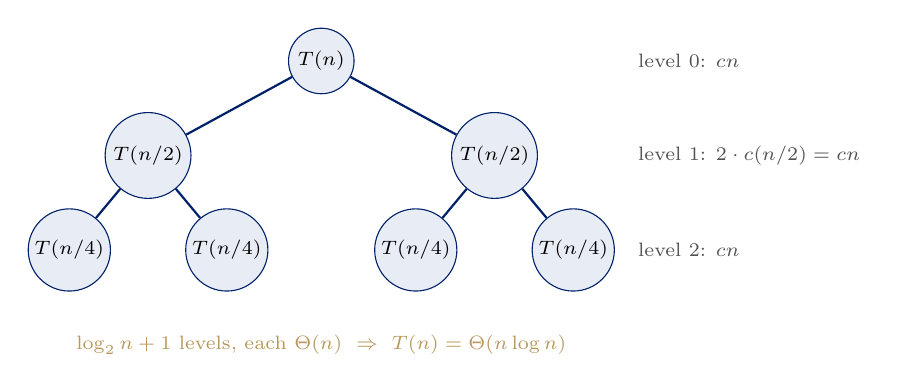
\begin{tikzpicture}[every node/.style={font=\scriptsize}]
    \node[circle, draw=primary-blue, fill=light-bg, inner sep=2pt]
      (t0) at (0, 3.2) {$T(n)$};
    \node[circle, draw=primary-blue, fill=light-bg, inner sep=2pt]
      (t1) at (-2.2, 2.0) {$T(n/2)$};
    \node[circle, draw=primary-blue, fill=light-bg, inner sep=2pt]
      (t2) at (2.2, 2.0) {$T(n/2)$};
    \foreach \x/\lab/\nm in {-3.2/{$T(n/4)$}/g1,-1.2/{$T(n/4)$}/g2,
                              1.2/{$T(n/4)$}/g3,3.2/{$T(n/4)$}/g4}
      \node[circle, draw=primary-blue, fill=light-bg, inner sep=1.5pt]
        (\nm) at (\x, 0.8) {\lab};
    \draw[thick, primary-blue] (t0) -- (t1);
    \draw[thick, primary-blue] (t0) -- (t2);
    \draw[thick, primary-blue] (t1) -- (g1);
    \draw[thick, primary-blue] (t1) -- (g2);
    \draw[thick, primary-blue] (t2) -- (g3);
    \draw[thick, primary-blue] (t2) -- (g4);
    \node[text=neutral, anchor=west] at (3.9, 3.2) {level $0$: $cn$};
    \node[text=neutral, anchor=west] at (3.9, 2.0) {level $1$: $2\cdot c(n/2) = cn$};
    \node[text=neutral, anchor=west] at (3.9, 0.8) {level $2$: $cn$};
    \node[text=primary-gold, align=center] at (0, -0.4)
      {$\log_2 n + 1$ levels, each $\Theta(n)$ $\;\Rightarrow\;$
        $T(n) = \Theta(n\log n)$};
  \end{tikzpicture}
  \caption{The recursion tree of merge sort: every level performs $\Theta(n)$ total merge work, and there are $\log_2 n + 1$ levels --- cf.\ \textit{Sedgewick}, Sec.~2.2, p.270 \cite{Sedgewick2011_algorithms}.}
\end{figure}

\begin{figure}[h]
  \centering
  % Diagram: merge sort of [38,27,43,3,9,82,10,19]. Four rows show the
  % split from one 8-cell array to eight singleton arrays; the merge phase
  % runs the same ladder upward. Cells 0.8 cm wide at x = 0..7.
  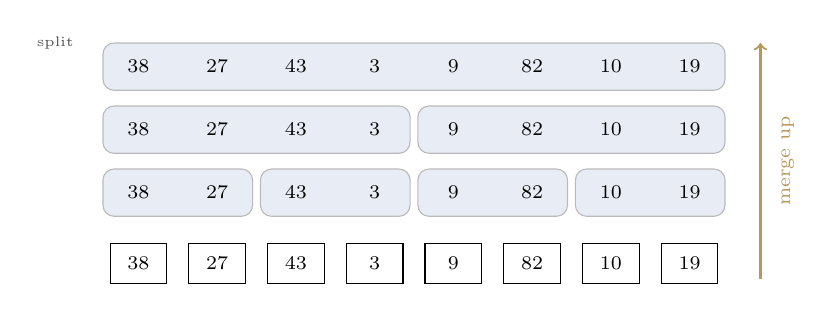
\begin{tikzpicture}[every node/.style={font=\scriptsize}]
    \draw[rounded corners, fill=light-bg, draw=neutral!40]
      (-0.45, 2.25) rectangle (7.45, 2.85);
    \foreach \i/\v in {0/38,1/27,2/43,3/3,4/9,5/82,6/10,7/19}
      \node at (\i, 2.55) {\v};
    \draw[rounded corners, fill=light-bg, draw=neutral!40]
      (-0.45, 1.45) rectangle (3.45, 2.05);
    \draw[rounded corners, fill=light-bg, draw=neutral!40]
      (3.55, 1.45) rectangle (7.45, 2.05);
    \foreach \i/\v in {0/38,1/27,2/43,3/3,4/9,5/82,6/10,7/19}
      \node at (\i, 1.75) {\v};
    \foreach \s in {0,2,4,6}
      \draw[rounded corners, fill=light-bg, draw=neutral!40]
        (\s-0.45, 0.65) rectangle (\s+1.45, 1.25);
    \foreach \i/\v in {0/38,1/27,2/43,3/3,4/9,5/82,6/10,7/19}
      \node at (\i, 0.95) {\v};
    \foreach \i/\v in {0/38,1/27,2/43,3/3,4/9,5/82,6/10,7/19}
      \node[draw, fill=white, minimum width=0.72cm, minimum height=0.5cm,
        inner sep=0] at (\i, 0.05) {\v};
    \draw[->, thick, primary-gold] (7.9, -0.15) -- (7.9, 2.85);
    \node[text=primary-gold, rotate=90, anchor=south] at (8.45, 1.35)
      {merge up};
    \node[text=neutral, anchor=east] at (-0.7, 2.85) {\tiny split};
  \end{tikzpicture}
  \caption{Splitting is index arithmetic and costs nothing; all the work is in the upward merges, each level merging every element once --- cf.\ \textit{Sedgewick}, Sec.~2.2, p.270 \cite{Sedgewick2011_algorithms}.}
\end{figure}

\subsection{Merge sort's bill}

Merge sort is $\Theta(n\log n)$ in the best, average, and worst cases. Even an already-sorted input must be merged, so there is no early exit and no input shape that helps or hurts: the cost is predictable. It is stable (ties take the left run) and predictable, which is worth real money in a library sort. It is not in-place: it needs a $\Theta(n)$ auxiliary buffer plus a $\Theta(\log n)$ recursion stack.

Its other virtue is structural. Merging two \emph{linked lists} needs no buffer at all --- just pointer splicing, the operation Week~7 built. That is why merge sort, not quick sort, is the model for external sorting in Week~10: when the data lives on disk, sequential merges are the natural unit of work.

\section{Partition: Quick Sort}

\textbf{Read alongside:} Sedgewick, Sec.~2.3, pp.288--307 --- quicksort; Wirth, Sec.~2.3.3, p.57 --- partition sort; Karumanchi, Ch.~10, pp.504--546 (PDF).

\subsection{The partition idea}

Merge sort does its work \emph{after} the recursion, in the merge. Quick sort does its work \emph{before}. It chooses one element as a \key{pivot}, rearranges the array so that everything at most the pivot sits to its left and everything greater sits to its right, then recurses on the two sides. There is no merge step. Once the pivot is placed, it is in its final position and never moves again.

\begin{definitionbox}{partition \cite{Wirth2004_algorithms_data_structures,Sedgewick2011_algorithms}}
Choose a pivot $p$. Rearrange $A[\texttt{lo}..\texttt{hi}]$ so that some index $q$ holds $p$, every element of $A[\texttt{lo}..q-1]$ is at most $p$, and every element of $A[q+1..\texttt{hi}]$ is greater than $p$. Return $q$. The partition is one linear pass, $\Theta(n)$, with $O(1)$ extra space.
\end{definitionbox}

The recurrence therefore has the same shape as merge sort's,
\[
  T(n) = T(k) + T(n-1-k) + \Theta(n),
\]
where $k$ is the size of the left part. But $k$ is now data-dependent, and that is where the danger lives.

\subsection{Lomuto partition}

\begin{verbatim}
int partition(int A[], int lo, int hi) {
  int pivot = A[hi];            // last element as the pivot
  int i = lo - 1;               // boundary of the <= pivot region
  for (int j = lo; j < hi; j++)
    if (A[j] <= pivot) {        // <= keeps equal keys on the left
      i++;
      swap(&A[i], &A[j]);
    }
  swap(&A[i + 1], &A[hi]);      // pivot into its final slot
  return i + 1;
}
\end{verbatim}

The invariant before each iteration is: $A[\texttt{lo}..i]$ holds elements at most the pivot, $A[i+1..j-1]$ holds elements greater than it, and $A[\texttt{hi}]$ holds the pivot. Each element is examined once, so the pass is $\Theta(n)$ with $O(1)$ extra space.

\begin{example}
Partition $[7,2,9,4,3,8,5]$ with pivot $5$ (the last element).
Start with $i=-1$.
$j=0$: $7>5$, no move.
$j=1$: $2\le5$, so $i=0$ and swap $A[0],A[1]$: $[2,7,9,4,3,8,5]$.
$j=2$: $9>5$, no move.
$j=3$: $4\le5$, so $i=1$ and swap $A[1],A[3]$: $[2,4,9,7,3,8,5]$.
$j=4$: $3\le5$, so $i=2$ and swap $A[2],A[4]$: $[2,4,3,7,9,8,5]$.
$j=5$: $8>5$, no move.
Finally swap $A[i+1]=A[3]$ with $A[6]$: $[2,4,3,5,9,8,7]$. The pivot $5$ is at index $3$; the left side $\{2,4,3\}$ is at most $5$, the right side $\{9,8,7\}$ is greater.
\end{example}

\begin{figure}[h]
  \centering
  % Diagram: Lomuto partition of [7,2,9,4,3,8,5] with pivot 5.
  % Three rows: initial, after j=4, final. Cells at x = 0..6 (1 cm apart),
  % rows y = 1.5, 0.4, -0.7. Green = <= pivot region, gold = pivot.
  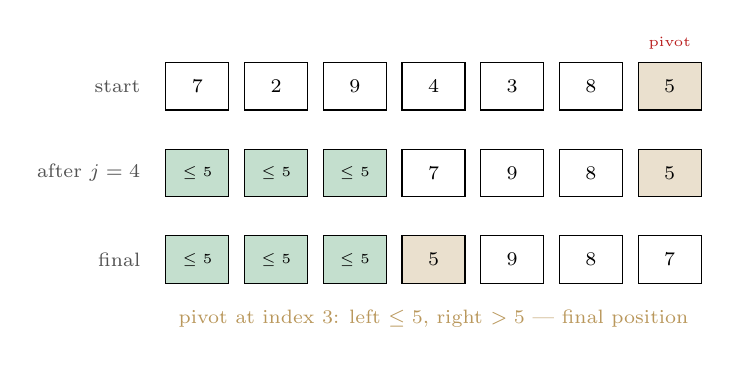
\begin{tikzpicture}[every node/.style={font=\scriptsize}]
    \foreach \i/\v in {0/7,1/2,2/9,3/4,4/3,5/8,6/5}
      \node[draw, fill=white, minimum width=0.8cm, minimum height=0.6cm,
        align=center] at (\i, 1.5) {\v};
    \node[draw, fill=primary-gold!30, minimum width=0.8cm,
      minimum height=0.6cm, align=center] at (6, 1.5) {5};
    \node[anchor=east, text=neutral] at (-0.6, 1.5) {start};
    \node[text=negative, anchor=south] at (6, 1.85) {\tiny pivot};
    \foreach \i/\v in {0/2,1/4,2/3,3/7,4/9,5/8,6/5}
      \node[draw, fill=white, minimum width=0.8cm, minimum height=0.6cm,
        align=center] at (\i, 0.4) {\v};
    \foreach \i in {0,1,2}
      \node[draw, fill=positive!25, minimum width=0.8cm,
        minimum height=0.6cm, align=center] at (\i, 0.4) {\tiny $\le 5$};
    \node[draw, fill=primary-gold!30, minimum width=0.8cm,
      minimum height=0.6cm, align=center] at (6, 0.4) {5};
    \node[anchor=east, text=neutral] at (-0.6, 0.4) {after $j=4$};
    \foreach \i/\v in {0/2,1/4,2/3,3/5,4/9,5/8,6/7}
      \node[draw, fill=white, minimum width=0.8cm, minimum height=0.6cm,
        align=center] at (\i, -0.7) {\v};
    \foreach \i in {0,1,2}
      \node[draw, fill=positive!25, minimum width=0.8cm,
        minimum height=0.6cm, align=center] at (\i, -0.7) {\tiny $\le 5$};
    \node[draw, fill=primary-gold!30, minimum width=0.8cm,
      minimum height=0.6cm, align=center] at (3, -0.7) {5};
    \node[anchor=east, text=neutral] at (-0.6, -0.7) {final};
    \node[text=primary-gold, align=center] at (3.0, -1.45)
      {pivot at index $3$: left $\le 5$, right $> 5$ --- final position};
  \end{tikzpicture}
  \caption{One Lomuto partition of $[7,2,9,4,3,8,5]$ around $5$. The green region is at most the pivot; the final swap places the pivot at index $3$ --- cf.\ \textit{Wirth}, Sec.~2.3.3, p.57 \cite{Wirth2004_algorithms_data_structures}.}
\end{figure}

\subsection{The recursive algorithm}

\begin{verbatim}
void qsortRange(int A[], int lo, int hi) {
  while (lo < hi) {                 // loop = tail-call elimination
    int p = partition(A, lo, hi);
    if (p - lo < hi - p) {          // recurse on the SMALLER side
      qsortRange(A, lo, p - 1);
      lo = p + 1;                   // iterate on the larger side
    } else {
      qsortRange(A, p + 1, hi);
      hi = p - 1;
    }
  }
}
\end{verbatim}

The \texttt{while} loop replaces a tail call, and recursing on the smaller side first bounds the stack depth to $O(\log n)$ even when the splits are badly unbalanced. After the partition, both recursive calls see strictly smaller ranges, so the recursion terminates.

\subsection{Best and average cases}

If every pivot lands near the middle, the two sides have about $n/2$ elements and the recurrence is merge sort's:
\[
  T(n) = 2\,T(n/2) + \Theta(n) = \Theta(n\log n).
\]
The average case over random pivots is also $\Theta(n\log n)$. More strongly, the splits need not be even. With a $9{:}1$ split at every level,
\[
  T(n) = T(9n/10) + T(n/10) + \Theta(n) = \Theta(n\log n).
\]
The reason is that each level still performs $\Theta(n)$ total work; only the number of levels grows, and it stays $\Theta(\log n)$ as long as every split removes a constant fraction of the data. Constant-factor imbalance is harmless. A split that removes only \emph{one} element is not.

\subsection{The worst case}

Take the sorted array $[1,2,3,4,5,6]$ and the code above. The pivot is always \texttt{A[hi]}, which is always the largest remaining element. The partition then produces a left side of $n-1$ elements and a right side of $0$. The recurrence collapses to
\[
  T(n) = T(n-1) + \Theta(n) = \Theta(n^2),
\]
because the levels form a chain of lengths $n, n-1, \dots, 1$ rather than a tree of depth $\log n$.

\begin{figure}[h]
  \centering
  % Diagram: the chain of partitions for sorted input. Each row shows the
  % live range; the gold cell is the pivot, placed at the right end.
  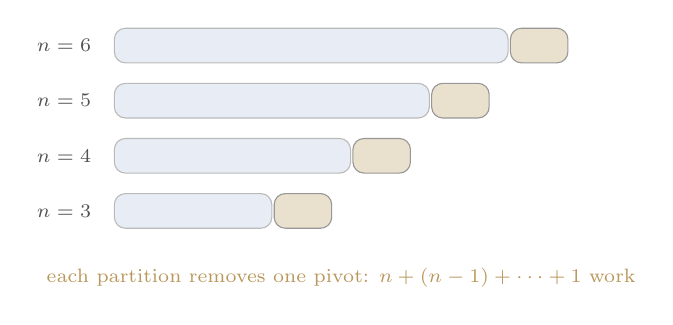
\begin{tikzpicture}[every node/.style={font=\scriptsize}]
    \draw[rounded corners, fill=light-bg, draw=neutral!40]
      (-0.38, 1.18) rectangle (4.62, 1.62);
    \draw[rounded corners, fill=primary-gold!30, draw=neutral!60]
      (4.65, 1.18) rectangle (5.38, 1.62);
    \node[anchor=east, text=neutral] at (-0.55, 1.4) {$n=6$};
    \draw[rounded corners, fill=light-bg, draw=neutral!40]
      (-0.38, 0.48) rectangle (3.62, 0.92);
    \draw[rounded corners, fill=primary-gold!30, draw=neutral!60]
      (3.65, 0.48) rectangle (4.38, 0.92);
    \node[anchor=east, text=neutral] at (-0.55, 0.7) {$n=5$};
    \draw[rounded corners, fill=light-bg, draw=neutral!40]
      (-0.38, -0.22) rectangle (2.62, 0.22);
    \draw[rounded corners, fill=primary-gold!30, draw=neutral!60]
      (2.65, -0.22) rectangle (3.38, 0.22);
    \node[anchor=east, text=neutral] at (-0.55, 0.0) {$n=4$};
    \draw[rounded corners, fill=light-bg, draw=neutral!40]
      (-0.38, -0.92) rectangle (1.62, -0.48);
    \draw[rounded corners, fill=primary-gold!30, draw=neutral!60]
      (1.65, -0.92) rectangle (2.38, -0.48);
    \node[anchor=east, text=neutral] at (-0.55, -0.7) {$n=3$};
    \node[text=primary-gold, align=center] at (2.5, -1.55)
      {each partition removes one pivot: $n + (n-1) + \cdots + 1$ work};
  \end{tikzpicture}
  \caption{Sorted input with a last-element pivot: every partition strips off one element, producing a chain of ranges rather than a balanced tree --- cf.\ \textit{Sedgewick}, Sec.~2.3, p.288 \cite{Sedgewick2011_algorithms}.}
\end{figure}

This worst case is not exotic. Sorted input is exactly what the calculator's identifier table is after the tokenizer has run, so a naive quicksort would undo the point of sorting.

\subsection{Choosing a pivot}

Two standard defences remove the natural bad inputs. \key{Median-of-three} takes the median of $A[\texttt{lo}]$, $A[\text{mid}]$, and $A[\texttt{hi}]$ as the pivot; on sorted or reverse-sorted input this picks the middle and restores balanced splits. \key{Randomization} swaps a uniformly random index into \texttt{hi} before partitioning; no fixed input can then force the worst case, and the expected cost over the algorithm's own randomness is $\Theta(n\log n)$.

Neither removes the $\Theta(n^2)$ worst case from the adversary's model, but median-of-three makes the common bad inputs good, and randomization makes the remaining bad cases astronomically unlikely. Practical libraries go further: \emph{introsort} runs quick sort, tracks recursion depth, and switches to heap sort when the depth exceeds $2\log_2 n$ --- quick sort's speed with heap sort's guarantee.

\subsection{Quick sort's bill}

Quick sort is $\Theta(n\log n)$ best and average, $\Theta(n^2)$ worst. It is in-place: $O(1)$ space for the partition and $O(\log n)$ recursion stack with the smaller-side rule, with no $\Theta(n)$ buffer. It is \bad{not stable} --- the long-range swaps leap equal keys over each other, exactly as selection sort did in Week~8. Its partition scans the array sequentially, so it is cache-friendly, which is why quick sort usually beats merge sort in wall-clock time despite the same $\Theta$ class and why it is the default general-purpose sort in most libraries.

\begin{example}
Quick sort $[1,2,3,4,5,6]$ with the last-element pivot. The first partition scans $5$ elements, the next $4$, then $3,2,1$. The total is
\[
  5+4+3+2+1 = 15 = \frac{n(n-1)}{2},
\]
which is $\Theta(n^2)$. With median-of-three on the same input the pivot is the middle element and the count drops to $\Theta(n\log n)$.
\end{example}

\section{The Comparison-Sort Lower Bound}

\textbf{Read alongside:} Aho--Hopcroft--Ullman, Ch.~8 (standard treatment) --- the comparison model and the sorting lower bound; Knuth, \textit{TAOCP} Vol.~3 (standard treatment).

\subsection{Count comparisons, not seconds}

Wall-clock time depends on the machine. The portable question is how many \emph{comparisons} a sort must make before it can be sure of the order. Every comparison sort --- insertion, merge, quick, heap --- learns about the data only by asking questions of the form ``is $A[i] < A[j]$?''. Each answer is yes or no.

A run on a fixed input therefore follows one path from the root of a \key{decision tree} to a leaf. Each internal node is one comparison; each leaf is the output permutation the algorithm believes. Only key comparisons are counted; moving, copying, and indexing are free.

\begin{definitionbox}{decision-tree model of a comparison sort \cite{AhoHopcroftUllman1983_data_structures_algorithms}}
A correct comparison sort must reach a \emph{different} leaf for each of the $n!$ possible input orderings. If two orderings ended at the same leaf, the algorithm would output the same permutation for both, and one of the two outputs would be wrong.
\end{definitionbox}

\subsection{The decision tree and the bound}

A binary tree with $L$ leaves has height at least $\lceil\log_2 L\rceil$. With $L=n!$ leaves, the worst-case number of comparisons is at least $\log_2(n!)$.

\begin{figure}[h]
  \centering
  % A full binary decision tree with six leaves, the count a correct
  % comparison sort of n=3 must distinguish. Every internal node has two
  % children (a comparison has two outcomes). Root at (0,3.0); height 3.
  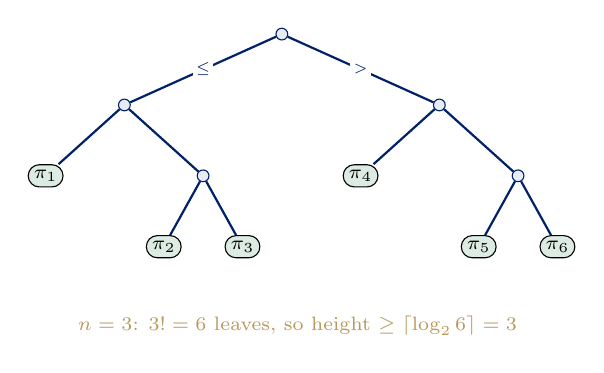
\begin{tikzpicture}[every node/.style={font=\scriptsize}]
    \node[circle, draw=primary-blue, fill=light-bg, inner sep=1.5pt]
      (r) at (0, 3.0) {};
    \node[circle, draw=primary-blue, fill=light-bg, inner sep=1.5pt]
      (l) at (-2.0, 2.1) {};
    \node[circle, draw=primary-blue, fill=light-bg, inner sep=1.5pt]
      (rr) at (2.0, 2.1) {};
    \node[draw, rounded corners, fill=positive!15, inner sep=2pt]
      (l1) at (-3.0, 1.2) {$\pi_1$};
    \node[circle, draw=primary-blue, fill=light-bg, inner sep=1.5pt]
      (l2) at (-1.0, 1.2) {};
    \node[draw, rounded corners, fill=positive!15, inner sep=2pt]
      (r1) at (1.0, 1.2) {$\pi_4$};
    \node[circle, draw=primary-blue, fill=light-bg, inner sep=1.5pt]
      (r2) at (3.0, 1.2) {};
    \node[draw, rounded corners, fill=positive!15, inner sep=2pt]
      (l21) at (-1.5, 0.3) {$\pi_2$};
    \node[draw, rounded corners, fill=positive!15, inner sep=2pt]
      (l22) at (-0.5, 0.3) {$\pi_3$};
    \node[draw, rounded corners, fill=positive!15, inner sep=2pt]
      (r21) at (2.5, 0.3) {$\pi_5$};
    \node[draw, rounded corners, fill=positive!15, inner sep=2pt]
      (r22) at (3.5, 0.3) {$\pi_6$};
    \draw[thick, primary-blue] (r) -- node[fill=white, inner sep=1pt,
      font=\tiny, text=primary-blue] {$\le$} (l);
    \draw[thick, primary-blue] (r) -- node[fill=white, inner sep=1pt,
      font=\tiny, text=primary-blue] {$>$} (rr);
    \draw[thick, primary-blue] (l) -- (l1);
    \draw[thick, primary-blue] (l) -- (l2);
    \draw[thick, primary-blue] (rr) -- (r1);
    \draw[thick, primary-blue] (rr) -- (r2);
    \draw[thick, primary-blue] (l2) -- (l21);
    \draw[thick, primary-blue] (l2) -- (l22);
    \draw[thick, primary-blue] (r2) -- (r21);
    \draw[thick, primary-blue] (r2) -- (r22);
    \node[text=primary-gold, align=center] at (0.2, -0.7)
      {$n=3$: $3! = 6$ leaves, so height $\ge \lceil\log_2 6\rceil = 3$};
  \end{tikzpicture}
  \caption{A decision tree for $n=3$ has six leaves, so its height --- the worst-case number of comparisons --- is at least $3$ --- cf.\ \textit{Aho--Hopcroft--Ullman}, Ch.~8 (standard treatment) \cite{AhoHopcroftUllman1983_data_structures_algorithms}.}
\end{figure}

To lower-bound $\log_2(n!)$, keep only the larger half of the factors:
\[
  \log_2(n!) = \sum_{k=1}^{n}\log_2 k
  \;\ge\; \sum_{k=\lceil n/2\rceil}^{n}\log_2\!\left(\frac{n}{2}\right)
  \;=\; \frac{n}{2}\log_2\!\left(\frac{n}{2}\right)
  \;=\; \Omega(n\log n).
\]
The matching upper bound is immediate, $\log_2(n!) \le n\log_2 n$, so $\log_2(n!) = \Theta(n\log n)$. Stirling's approximation gives the sharper form
\[
  \log_2(n!) = n\log_2 n - \frac{n}{\ln 2} + O(\log n)
  \approx n\log_2 n - 1.44\,n.
\]

\begin{definitionbox}{comparison-sort lower bound \cite{AhoHopcroftUllman1983_data_structures_algorithms,Knuth1998_taocp_volume3}}
Every comparison sort makes at least $\Omega(n\log n)$ comparisons in the worst case. Merge sort and heap sort reach this bound, which is why they are optimal among comparison sorts.
\end{definitionbox}

\subsection{What the wall does and does not say}

The bound is a \emph{worst-case} statement over all inputs. An adaptive sort can be $O(n)$ on a particular input --- insertion sort on sorted data does $n-1$ comparisons --- but some input still forces $\Omega(n\log n)$. It applies only to algorithms that learn about keys by comparing them, so it says nothing about a sort that reads the bits of a key directly. And it does not say $n\log n$ is the fastest possible sorting time; it says $n\log n$ is the fastest possible \emph{comparison} sorting time.

As a sanity check, $10! = 3{,}628{,}800$ and $\log_2(10!) \approx 22$, while $10\log_2 10 \approx 33$; for $20$ elements, $20! \approx 2.4\times10^{18}$ and $\log_2(20!) \approx 61$. The constants are not tight for small $n$; the asymptotic statement is what matters.

\section{Heap Sort: The Guarantee in Constant Space}

\textbf{Read alongside:} Karumanchi, Ch.~7, pp.369--408 (PDF), Sec.~7.7 --- heaps and heapsort; Sedgewick, Sec.~2.4, pp.308--335 --- priority queues and heapsort.

\subsection{An array that thinks it is a tree}

Merge sort has the guarantee but pays $\Theta(n)$ space; quick sort has the space but loses the guarantee. Heap sort has both, by storing a \emph{complete binary tree} in the array itself with no pointers.

\begin{definitionbox}{binary max-heap \cite{Karumanchi2017_data_structures_algorithms_made_easy,Sedgewick2011_algorithms}}
A binary max-heap is a complete binary tree with the \key{heap property}: for every node $i$, $A[i]\ge A[\text{left}(i)]$ and $A[i]\ge A[\text{right}(i)]$. In a 0-based array, $\text{left}(i)=2i+1$, $\text{right}(i)=2i+2$, and $\text{parent}(i)=\lfloor(i-1)/2\rfloor$. The maximum is always $A[0]$.
\end{definitionbox}

The tree structure is pure index arithmetic --- the same address arithmetic as Week~3's arrays --- which is what makes $O(1)$ space possible.

\begin{figure}[h]
  \centering
  % Diagram: max-heap [50,30,40,10,20,35,25] drawn as a tree over the same
  % array. Tree root (0,2.5), children (+-1.6,1.6), grandchildren
  % (-2.4,-0.8,0.8,2.4 at y=0.7). Array cells at x = 0..6, y = -0.6.
  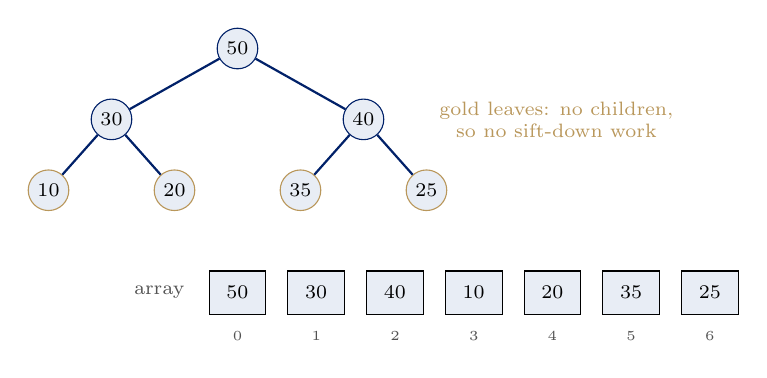
\begin{tikzpicture}[every node/.style={font=\scriptsize}]
    \node[circle, draw=primary-blue, fill=light-bg, inner sep=2pt]
      (n0) at (0, 2.5) {50};
    \node[circle, draw=primary-blue, fill=light-bg, inner sep=2pt]
      (n1) at (-1.6, 1.6) {30};
    \node[circle, draw=primary-blue, fill=light-bg, inner sep=2pt]
      (n2) at (1.6, 1.6) {40};
    \node[circle, draw=primary-gold, fill=light-bg, inner sep=2pt]
      (n3) at (-2.4, 0.7) {10};
    \node[circle, draw=primary-gold, fill=light-bg, inner sep=2pt]
      (n4) at (-0.8, 0.7) {20};
    \node[circle, draw=primary-gold, fill=light-bg, inner sep=2pt]
      (n5) at (0.8, 0.7) {35};
    \node[circle, draw=primary-gold, fill=light-bg, inner sep=2pt]
      (n6) at (2.4, 0.7) {25};
    \foreach \a/\b in {n0/n1,n0/n2,n1/n3,n1/n4,n2/n5,n2/n6}
      \draw[thick, primary-blue] (\a) -- (\b);
    \foreach \i/\v in {0/50,1/30,2/40,3/10,4/20,5/35,6/25}
      \node[draw, fill=light-bg, minimum width=0.72cm,
        minimum height=0.55cm, inner sep=0] at (\i, -0.6) {\v};
    \foreach \i in {0,...,6}
      \node[text=neutral] at (\i, -1.15) {\tiny \i};
    \node[text=neutral, anchor=east] at (-0.55, -0.6) {array};
    \node[text=primary-gold, align=center] at (4.05, 1.6)
      {gold leaves: no children,\\ so no sift-down work};
  \end{tikzpicture}
  \caption{A max-heap of seven values in an array: $50\ge30,40$; $30\ge10,20$; $40\ge35,25$. The leaves need no sift-down work --- cf.\ \textit{Karumanchi}, Ch.~7, pp.369--408 (PDF) \cite{Karumanchi2017_data_structures_algorithms_made_easy}.}
\end{figure}

\subsection{Sift down}

Restoring the heap property after a change means pushing an element down until it is at least as large as both children:

\begin{verbatim}
void siftDown(int A[], int i, int n) {
  for (;;) {
    int l = 2 * i + 1, r = l + 1, m = i;
    if (l < n && A[l] > A[m]) m = l;   // larger child
    if (r < n && A[r] > A[m]) m = r;
    if (m == i) return;                // heap property restored
    swap(&A[i], &A[m]);
    i = m;                             // keep sinking
  }
}
\end{verbatim}

Only one subtree can violate the property after a swap, so each call follows a single root-to-leaf path: at most $\lfloor\log_2 n\rfloor$ swaps.

\subsection{Building a heap in $\Theta(n)$}

The obvious build performs $n$ insertions, each sifting up in $O(\log n)$, for $O(n\log n)$ total. It is correct but not tight. The tight build sifts \emph{down} every internal node, from the last parent $\lfloor n/2\rfloor-1$ back to index $0$; leaves need no work.

Count the work by height. About $n/2$ nodes are leaves (height $0$), $n/4$ have height $1$, $n/8$ height $2$, and so on:
\[
  \sum_{h\ge0}\frac{n}{2^{h+1}}\,h
  = \frac{n}{2}\sum_{h\ge0}\frac{h}{2^{h}}
  = \frac{n}{2}\cdot 2
  = \Theta(n).
\]
Half the nodes never move, a quarter move at most one level, an eighth at most two. The expensive top-of-tree nodes are few. This is the classic case where the obvious bound is off by a log factor --- the amortized-counting habit Week~2 built.

\subsection{The algorithm and its bill}

\begin{verbatim}
void heapSort(int A[], int n) {
  for (int i = n / 2 - 1; i >= 0; i--)   // build max-heap: Theta(n)
    siftDown(A, i, n);
  for (int end = n - 1; end > 0; end--) {
    swap(&A[0], &A[end]);                // max to its final slot
    siftDown(A, 0, end);                 // restore on the shrinking heap
  }
}
\end{verbatim}

Phase~1 is $\Theta(n)$ by the height sum. Phase~2 performs $n-1$ extractions, each $O(\log n)$, for $\Theta(n\log n)$. The total is $\Theta(n\log n)$ in the worst case with $\Theta(1)$ auxiliary space --- a combination unique among the sorts in this course.

Heap sort is \bad{not stable} (long-range swaps across the heap) and \bad{not cache-friendly}: sift-down jumps by powers of two across the array, so each access lands far from the previous one. That is why quick sort is often several times faster in practice despite the same $\Theta$ class. Heap sort's niche is exactly where the guarantee and the memory bound matter: real-time and embedded systems, and introsort's fallback.

\section{Radix Sort: Leaving the Comparison Model}

\textbf{Read alongside:} Sedgewick, Sec.~5.1, p.702 --- string sorts and LSD radix; Karumanchi, Ch.~10, pp.504--546 (PDF) --- radix sort.

The lower bound assumed that the only thing a sort may do is compare two whole keys. But a three-digit number already says a lot about where it belongs: the hundreds digit is more significant than the tens. Radix sort exploits that structure.

\begin{definitionbox}{LSD radix sort \cite{Sedgewick2011_algorithms,Karumanchi2017_data_structures_algorithms_made_easy}}
For $d$ digits and a base-$k$ alphabet, run a \emph{stable} counting sort on digit $0$ (units), then digit $1$ (tens), up to digit $d-1$. After pass $t$, the array is sorted by its last $t+1$ digits; after the final pass it is fully sorted.
\end{definitionbox}

The passes must go least-significant first, and each must be stable: a later, more-significant pass must not disturb the order the earlier passes established within equal digits.

\begin{example}
Sort $[170,45,75,90,802,24]$ in base $10$ over three digits.
\textbf{Units pass} (stable): $170,90$ end in $0$; $802,24$ have units $2,4$; $45,75$ end in $5$. Result: $[170,90,802,24,45,75]$.
\textbf{Tens pass} (stable): tens digits are $7,9,0,2,4,7$. Group in increasing digit, preserving order within a group: $[802,24,45,75,170,90]$.
\textbf{Hundreds pass} (stable): hundreds digits are $8,0,0,0,1,0$. Result: $[24,45,75,90,170,802]$. The array is sorted.
\end{example}

\begin{figure}[h]
  \centering
  % Diagram: LSD radix sort of [170,45,75,90,802,24], base 10, 3 digits.
  % Four rows: input, after units, after tens, after hundreds. Cells 1.1 cm
  % wide at x = 0..5; rows y = 2.5, 1.6, 0.7, -0.2.
  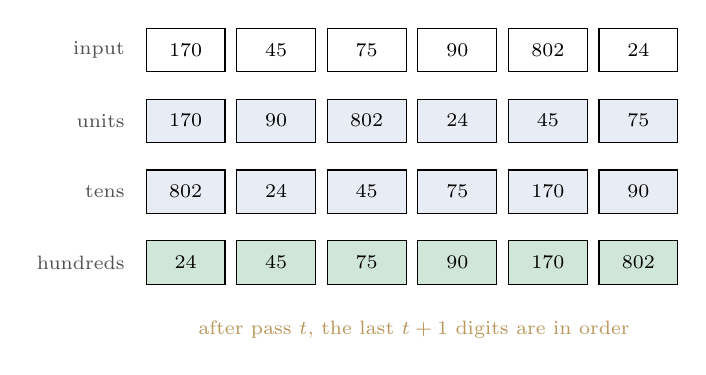
\begin{tikzpicture}[every node/.style={font=\scriptsize}]
    \foreach \i/\v in {0/170,1/45,2/75,3/90,4/802,5/24}
      \node[draw, fill=white, minimum width=1.0cm, minimum height=0.55cm,
        inner sep=1pt] at (\i*1.15, 2.5) {\v};
    \node[anchor=east, text=neutral] at (-0.65, 2.5) {input};
    \foreach \i/\v in {0/170,1/90,2/802,3/24,4/45,5/75}
      \node[draw, fill=light-bg, minimum width=1.0cm,
        minimum height=0.55cm, inner sep=1pt] at (\i*1.15, 1.6) {\v};
    \node[anchor=east, text=neutral] at (-0.65, 1.6) {units};
    \foreach \i/\v in {0/802,1/24,2/45,3/75,4/170,5/90}
      \node[draw, fill=light-bg, minimum width=1.0cm,
        minimum height=0.55cm, inner sep=1pt] at (\i*1.15, 0.7) {\v};
    \node[anchor=east, text=neutral] at (-0.65, 0.7) {tens};
    \foreach \i/\v in {0/24,1/45,2/75,3/90,4/170,5/802}
      \node[draw, fill=positive!20, minimum width=1.0cm,
        minimum height=0.55cm, inner sep=1pt] at (\i*1.15, -0.2) {\v};
    \node[anchor=east, text=neutral] at (-0.65, -0.2) {hundreds};
    \node[text=primary-gold, align=center] at (2.9, -1.05)
      {after pass $t$, the last $t+1$ digits are in order};
  \end{tikzpicture}
  \caption{Three stable passes of LSD radix sort on $[170,45,75,90,802,24]$ --- cf.\ \textit{Sedgewick}, Sec.~5.1, p.702 \cite{Sedgewick2011_algorithms}.}
\end{figure}

\begin{verbatim}
void radixSort(int A[], int n, int digits, int base) {
  int *out = malloc(n * sizeof(int));
  for (int d = 0, div = 1; d < digits; d++, div *= base) {
    int count[10] = {0};                 // base <= 10 here
    for (int i = 0; i < n; i++)
      count[(A[i] / div) % base]++;
    for (int v = 1; v < base; v++) count[v] += count[v - 1];
    for (int i = n - 1; i >= 0; i--)     // reverse => stable
      out[--count[(A[i] / div) % base]] = A[i];
    for (int i = 0; i < n; i++) A[i] = out[i];
  }
  free(out);
}
\end{verbatim}

Each pass is Week~8's stable counting sort applied to one digit: tally, prefix sums, reverse scatter. The outer loop advances the digit.

The cost is $\Theta(d(n+k))$ time and $\Theta(n+k)$ space. For $32$-bit keys with $8$-bit digits, $d=4$ and $k=256$, so four linear passes suffice. Radix sort makes \emph{zero} comparisons of whole keys, so the $\Omega(n\log n)$ comparison bound does not apply to it. Its precondition is real, however: keys must have a positional representation with a known width --- integers or fixed-length strings. Arbitrary objects with only a comparison function cannot use it. The lesson is that a lower bound is only as strong as its model; radix sort does not break the mathematics, it changes the question from ``compare two keys'' to ``read one digit''.

\section{Shell Sort: Diminishing Increments}

\textbf{Read alongside:} Wirth, Sec.~2.3.1, p.52 --- insertion sort by diminishing increment; Sedgewick, Sec.~2.1, p.244 --- elementary sorts; Karumanchi, Ch.~10, pp.504--546 (PDF).

Insertion sort is $O(n)$ on nearly-sorted input and $\Theta(n^2)$ on random input. Shell sort manufactures ``nearly sorted'' cheaply: it insertion-sorts widely spaced subsequences first, then narrows the spacing.

\begin{definitionbox}{diminishing-increment sort \cite{Wirth2004_algorithms_data_structures,Sedgewick2011_algorithms}}
Choose a decreasing \key{gap sequence} $h_1>h_2>\cdots>h_t=1$. For each gap $h$, insertion-sort every subsequence $A[i],A[i+h],A[i+2h],\dots$. The final pass with $h=1$ is ordinary insertion sort, so correctness is automatic.
\end{definitionbox}

A gap of $n/2$ can move an element halfway across the array in one shift. By the time $h=1$, few inversions remain, so the final insertion pass is close to linear. Shell's original sequence $n/2,n/4,\dots,1$ is simple but has a $\Theta(n^2)$ worst case; Knuth's $(3^k-1)/2$ sequence gives $O(n^{3/2})$, and Sedgewick's gives $O(n^{4/3})$. No sequence is known to be optimal.

\begin{example}
Sort $[7,3,9,1,8,2,6,4]$ with gaps $4$, then $2$, then $1$.
\textbf{Gap $4$:} the subsequences are $(7,8)$, $(3,2)$, $(9,6)$, $(1,4)$; each is already sorted or swapped into order, giving $(7,8)$, $(2,3)$, $(6,9)$, $(1,4)$, i.e.\ $[7,2,6,1,8,3,9,4]$.
\textbf{Gap $2$:} the even positions hold $[7,6,8,9]$, sorted to $[6,7,8,9]$; the odd positions hold $[2,1,3,4]$, sorted to $[1,2,3,4]$. The array becomes $[6,1,7,2,8,3,9,4]$.
\textbf{Gap $1$:} ordinary insertion sort gives $[1,2,3,4,6,7,8,9]$.
\end{example}

\begin{figure}[h]
  \centering
  % Diagram: shell sort of [7,3,9,1,8,2,6,4] with gaps 4, 2, 1.
  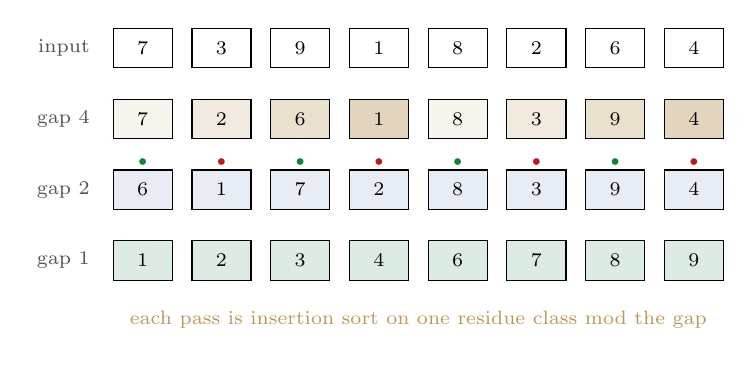
\begin{tikzpicture}[every node/.style={font=\scriptsize}]
    \foreach \i/\v in {0/7,1/3,2/9,3/1,4/8,5/2,6/6,7/4}
      \node[draw, fill=white, minimum width=0.75cm, minimum height=0.5cm,
        inner sep=0] at (\i, 2.4) {\v};
    \node[anchor=east, text=neutral] at (-0.55, 2.4) {input};
    \foreach \i/\v/\c in {0/7/1,1/2/2,2/6/3,3/1/4,4/8/1,5/3/2,6/9/3,7/4/4}
      \node[draw, fill=primary-gold!\c0, minimum width=0.75cm,
        minimum height=0.5cm, inner sep=0] at (\i, 1.5) {\v};
    \node[anchor=east, text=neutral] at (-0.55, 1.5) {gap $4$};
    \foreach \i/\v in {0/6,1/1,2/7,3/2,4/8,5/3,6/9,7/4}
      \node[draw, fill=light-bg, minimum width=0.75cm,
        minimum height=0.5cm, inner sep=0] at (\i, 0.6) {\v};
    \foreach \i in {0,2,4,6}
      \node[text=positive] at (\i, 0.95) {\tiny $\bullet$};
    \foreach \i in {1,3,5,7}
      \node[text=negative] at (\i, 0.95) {\tiny $\bullet$};
    \node[anchor=east, text=neutral] at (-0.55, 0.6) {gap $2$};
    \foreach \i/\v in {0/1,1/2,2/3,3/4,4/6,5/7,6/8,7/9}
      \node[draw, fill=positive!15, minimum width=0.75cm,
        minimum height=0.5cm, inner sep=0] at (\i, -0.3) {\v};
    \node[anchor=east, text=neutral] at (-0.55, -0.3) {gap $1$};
    \node[text=primary-gold, align=center] at (3.5, -1.05)
      {each pass is insertion sort on one residue class mod the gap};
  \end{tikzpicture}
  \caption{Shell sort with gaps $4,2,1$: each pass insertion-sorts one residue class modulo the gap --- cf.\ \textit{Wirth}, Sec.~2.3.1, p.52 \cite{Wirth2004_algorithms_data_structures}.}
\end{figure}

\begin{verbatim}
void shellSort(int A[], int n) {
  for (int gap = n / 2; gap > 0; gap /= 2) {  // Shell's halving sequence
    for (int i = gap; i < n; i++) {
      int key = A[i], j = i;
      while (j >= gap && A[j - gap] > key) {  // shifted insertion
        A[j] = A[j - gap];
        j -= gap;
      }
      A[j] = key;
    }
  }
}
\end{verbatim}

Compare this with Week~8's insertion sort: the only change is the stride \texttt{gap} in place of $1$. With \texttt{gap = 1} the code is exactly the old insertion sort, which is the correctness argument. Shell sort is in-place and unstable, and simpler than quick sort, but its worst case depends on the gap sequence, so it carries no guarantee.

\section{Comparative Analysis and Choosing}

\textbf{Read alongside:} Wirth, Sec.~2.3.5, p.62 --- comparison of array sorting methods; Karumanchi, Ch.~10, pp.504--546 (PDF) --- the comparison-of-sorting-algorithms table.

\begin{center}
{\footnotesize
\begin{tabular}{l l l l l c c}
  \toprule
  \textbf{sort} & \textbf{best} & \textbf{average} & \textbf{worst} &
    \textbf{space} & \textbf{stable} & \textbf{in-place} \\
  \midrule
  merge & $\Theta(n\log n)$ & $\Theta(n\log n)$ & $\Theta(n\log n)$ &
    $\Theta(n)$ & yes & no \\
  quick & $\Theta(n\log n)$ & $\Theta(n\log n)$ & $\Theta(n^2)$ &
    $O(\log n)$ & no & yes \\
  heap & $\Theta(n\log n)$ & $\Theta(n\log n)$ & $\Theta(n\log n)$ &
    $O(1)$ & no & yes \\
  shell & $O(n\log n)$ & depends on gaps & $\Theta(n^2)$ / $O(n^{3/2})$ &
    $O(1)$ & no & yes \\
  radix & $\Theta(d(n+k))$ & $\Theta(d(n+k))$ & $\Theta(d(n+k))$ &
    $\Theta(n+k)$ & yes & no \\
  \bottomrule
\end{tabular}}
\end{center}

The shell row's two worst-case entries are Shell's halving sequence ($\Theta(n^2)$) and Knuth's $(3^k-1)/2$ sequence ($O(n^{3/2})$); the cost is a property of the gap sequence, not of ``shell sort'' alone. Read the table by which cell is guaranteed: only merge and heap guarantee $\Theta(n\log n)$, and only heap combines that with $O(1)$ space.

The choice is a workload question, not a ranking. Worst-case guarantee with tight memory calls for heap sort. Raw average speed, in-place and cache-friendly, calls for quick sort with a randomized pivot. Stability, or linked and external data, calls for merge sort. Fixed-width integer or string keys with a known range call for radix sort. Nearly sorted input, or small $n$, calls for insertion sort; and simple in-place operation with no guarantee required calls for shell sort. The properties that decide it are the same three Week~8 introduced --- the case, stability, and space --- plus the guarantee that a $\Theta(n\log n)$ worst case is even possible.

\subsection*{Three classic mistakes}

\begin{itemize}
  \item \bad{``Quick sort is $O(n\log n)$'' with no case.} Its worst case is $\Theta(n^2)$, and the input that triggers it (sorted data with a last-element pivot) is exactly the input a tokenizer produces. State the case, then name the pivot rule.
  \item \bad{``Merge sort is in-place'' / ``quick sort is $O(1)$ space''.} Merge sort needs a $\Theta(n)$ buffer; quick sort needs an $O(\log n)$ recursion stack. Heap sort is the one efficient sort that is genuinely $O(1)$ auxiliary.
  \item \bad{``Radix sort is $O(n)$, so it always beats merge sort.''} It is $\Theta(d(n+k))$, linear only when $d$ and $k$ are treated as constants, and it needs $\Theta(n+k)$ space and fixed-width keys.
\end{itemize}

\subsection*{Week 9 summary}

Divide and conquer gives merge sort: split, sort, merge, with $T(n)=2T(n/2)+\Theta(n)=\Theta(n\log n)$ in every case; stable, with $\Theta(n)$ space. Partition gives quick sort: $\Theta(n\log n)$ average, $\Theta(n^2)$ worst on sorted input with a last-element pivot; in-place and unstable, so randomize or use median-of-three. The comparison lower bound says every comparison sort needs $\Omega(n\log n)$ comparisons, because a decision tree must distinguish all $n!$ orders. Heap sort reaches the bound in $O(1)$ space; radix sort leaves the comparison model with stable digit passes, $\Theta(d(n+k))$; shell sort buys simplicity and in-place operation with a gap-dependent bound.

Next week the table is sorted and searchable in $O(\log n)$. Week~10 asks a stronger question: can we find a record in \emph{one} probe, without sorting at all? File organization, hash functions, and collision resolution.

\subsection*{Exercises}

Answer from the algorithms, then check against the Solutions block: run each trace on paper first.
\begin{enumerate}
  \item \textbf{Merge.} Merge the sorted runs $[4,9,13]$ and $[1,7,10]$ by the two-finger method: write the output after each comparison, count the comparisons, and say which elements were drained without a comparison.
  \item \textbf{Partition.} Run Lomuto partition on $[6,3,8,1,5,2,7]$ with pivot $7$ (the last element). Give the array after each swap that the \texttt{A[j] <= pivot} test triggers, then the final array and the returned index.
  \item \textbf{Quick-sort worst case.} Quick sort $[1,2,3,4,5]$ with the last-element pivot. Give the total number of comparisons made by \texttt{partition}, and explain which structural property of the input causes it.
  \item \textbf{Radix.} Sort $[31,4,15,20,9,48]$ in base $10$ over two digits with LSD radix sort. Give the array after the units pass and after the tens pass; explain why the units pass must be stable.
  \item \textbf{Heap.} Build a max-heap from $[12,5,9,2,7,4]$ using the linear-time build, then extract the maximum once and show the array and the heap property afterward.
\end{enumerate}

\subsection*{Solutions}

\begingroup\small
\begin{enumerate}
  \item Compare $4$ and $1$: take $1$; $4$ and $7$: take $4$; $9$ and $7$: take $7$; $9$ and $10$: take $9$; $13$ and $10$: take $10$; drain $13$. Output $[1,4,7,9,10,13]$; five comparisons, and $13$ was drained without one.
  \item Start $i=-1$. $j=0$: $6\le7$, $i=0$, swap $A[0],A[0]$ (no change): $[6,3,8,1,5,2,7]$. $j=1$: $3\le7$, $i=1$, swap $A[1],A[1]$: no change. $j=2$: $8>7$, no move. $j=3$: $1\le7$, $i=2$, swap $A[2],A[3]$: $[6,3,1,8,5,2,7]$. $j=4$: $5\le7$, $i=3$, swap $A[3],A[4]$: $[6,3,1,5,8,2,7]$. $j=5$: $2\le7$, $i=4$, swap $A[4],A[5]$: $[6,3,1,5,2,8,7]$. Final swap $A[5],A[6]$: $[6,3,1,5,2,7,8]$; returned index $5$.
  \item The first partition scans $4$ elements, then $3,2,1$: total $4+3+2+1=10$. Sorted ascending input with a last-element pivot makes the largest element the pivot every time, so each partition leaves a left side of $n-1$ and a right side of $0$ --- a chain, not a balanced tree.
  \item \textbf{Units:} $31,20,4,15,48,9$ $\to$ digits $1,0,4,5,8,9$: $[20,31,4,15,48,9]$. \textbf{Tens:} $4,9$ have tens $0$; $15$ has $1$; $20$ has $2$; $31$ has $3$; $48$ has $4$: $[4,9,15,20,31,48]$. The units pass must be stable so that, within equal tens digits, the order established by the units pass survives.
  \item Build from $[12,5,9,2,7,4]$: the last parent is index $2$. Sift down index $2$ ($9$ with child $4$): no change. Index $1$ ($5$ with children $2,7$): swap with $7$ $\to[12,7,9,2,5,4]$. Index $0$ ($12$ with children $7,9$): no change. Heap: $[12,7,9,2,5,4]$. Extract the maximum: swap $12$ and $4$, shrink to $5$ elements: $[4,7,9,2,5]$; sift down index $0$: swap with $9$ $\to[9,7,4,2,5]$; sift down index $2$: no child larger, stop. Result $[9,7,4,2,5]$ with the heap property intact.
\end{enumerate}
\endgroup

\bibliography{../../Bibliography_base}
\bibliographystyle{plain}
\end{document}
